\documentclass[10pt]{article}

\usepackage[margin=0.75in]{geometry}
\usepackage{amsmath, amssymb}
\usepackage{graphicx}
\usepackage[T1]{fontenc}
\usepackage{inconsolata}
\usepackage{titlesec}
\usepackage{fancyhdr}
\usepackage{microtype}
\usepackage{tikz}
\usetikzlibrary{arrows.meta,calc,patterns}

\graphicspath{{../}}

\setlength{\parindent}{0pt}
\setlength{\parskip}{4pt}
\renewcommand{\baselinestretch}{1.05}

\titleformat{\section}{\ttfamily\normalsize\bfseries\MakeUppercase}{\thesection}{0.6em}{}
\titlespacing*{\section}{0pt}{8pt}{2pt}
\titleformat{\subsection}{\ttfamily\small\MakeUppercase}{\thesubsection}{0.6em}{}
\titlespacing*{\subsection}{0pt}{6pt}{2pt}

\pagestyle{fancy}
\fancyhf{}
\renewcommand{\headrulewidth}{0pt}
\renewcommand{\footrulewidth}{0.5pt}
\fancyfoot[L]{\ttfamily\footnotesize SAUNA-EXISTING-CONDITIONS}
\fancyfoot[C]{\ttfamily\footnotesize REV \today}
\fancyfoot[R]{\ttfamily\footnotesize \thepage}

\tikzset{
  font=\ttfamily\scriptsize,
  >=Latex,
  wood/.style={draw=black, line width=0.5pt, fill=black!8},
  thin/.style={draw=black, line width=0.4pt},
  thick/.style={draw=black, line width=0.9pt},
  dim/.style={draw=black, line width=0.4pt, {Bar[width=4pt]}-{Bar[width=4pt]}},
  tbd/.style={draw=black, line width=0.4pt, dashed},
  lab/.style={font=\ttfamily\scriptsize, inner sep=1.5pt, fill=white},
}

\begin{document}

\noindent
\includegraphics[height=0.7cm]{logo}\hfill
{\ttfamily\normalsize\bfseries\MakeUppercase{Sauna --- Existing Conditions}}\quad
{\ttfamily\footnotesize\today}
\vspace{4pt}\hrule\vspace{6pt}

{\ttfamily\footnotesize
\begin{tabular}{@{}ll@{}}
Measured & 2026-09-07, interior stud face to stud face, inches \\
Dashed & not yet measured (TBD) \\
Origin & interior corner, left of door walking in \\
\end{tabular}
}

\section{Plan}

\begin{center}
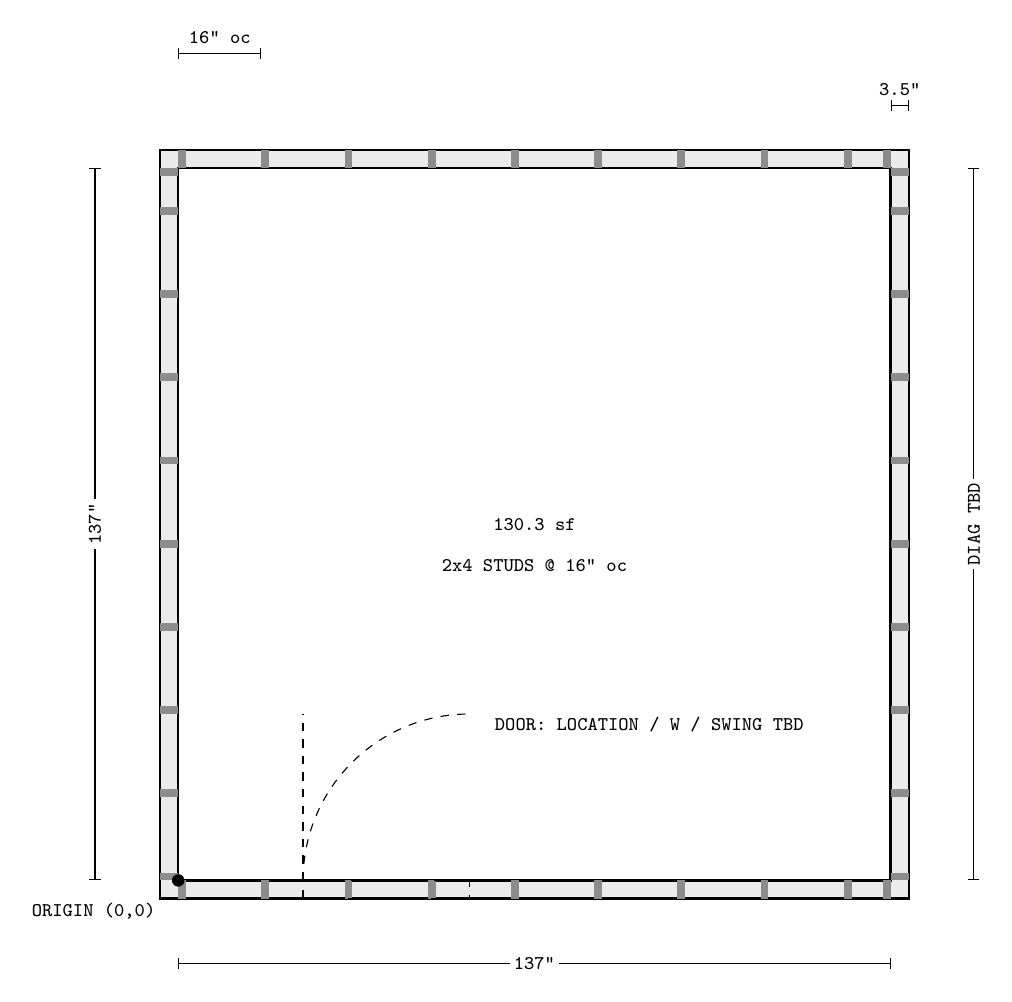
\begin{tikzpicture}[x=0.026in,y=0.026in]
% interior box 137 x 137; studs 3.5 deep outside it
\def\L{137}
\def\D{3.5}
% wall bands
\fill[black!8] (-\D,-\D) rectangle (\L+\D,\L+\D);
\fill[white] (0,0) rectangle (\L,\L);
\draw[thick] (-\D,-\D) rectangle (\L+\D,\L+\D);
\draw[thick] (0,0) rectangle (\L,\L);
% studs @16 oc, 1.5 wide, all four walls
\foreach \a in {0,16,...,128}{
  \fill[black!45] (\a,-\D) rectangle (\a+1.5,0);
  \fill[black!45] (\a,\L) rectangle (\a+1.5,\L+\D);
  \fill[black!45] (-\D,\a) rectangle (0,\a+1.5);
  \fill[black!45] (\L,\a) rectangle (\L+\D,\a+1.5);
}
\fill[black!45] (\L-1.5,-\D) rectangle (\L,0);
\fill[black!45] (\L-1.5,\L) rectangle (\L,\L+\D);
\fill[black!45] (-\D,\L-1.5) rectangle (0,\L);
\fill[black!45] (\L,\L-1.5) rectangle (\L+\D,\L);
% origin
\fill (0,0) circle (1.2);
\node[lab, anchor=north east] at (-\D,-\D) {ORIGIN (0,0)};
% door TBD on front wall
\draw[tbd] (24,-\D) rectangle (56,0);
\draw[tbd] (24,0) arc (180:90:32);
\draw[tbd] (24,0) -- (24,32);
\node[lab, anchor=west] at (60,30) {DOOR: LOCATION / W / SWING TBD};
% dims
\draw[dim] (0,-16) -- (\L,-16); \node[lab] at (\L/2,-16) {137"};
\draw[dim] (-16,0) -- (-16,\L); \node[lab, rotate=90] at (-16,\L/2) {137"};
\draw[dim] (\L+\D,\L+12) -- (\L,\L+12); \node[lab, anchor=south] at (\L+\D/2,\L+13) {3.5"};
\draw[dim] (0,\L+22) -- (16,\L+22); \node[lab, anchor=south] at (8,\L+23) {16" oc};
\draw[dim] (\L+16,0) -- (\L+16,\L); \node[lab, rotate=90] at (\L+16,\L/2) {DIAG TBD};
% area
\node[lab] at (\L/2,\L/2) {130.3 sf};
\node[lab, anchor=north] at (\L/2,\L/2-6) {2x4 STUDS @ 16" oc};
\end{tikzpicture}
\end{center}

\section{Section}

\begin{center}
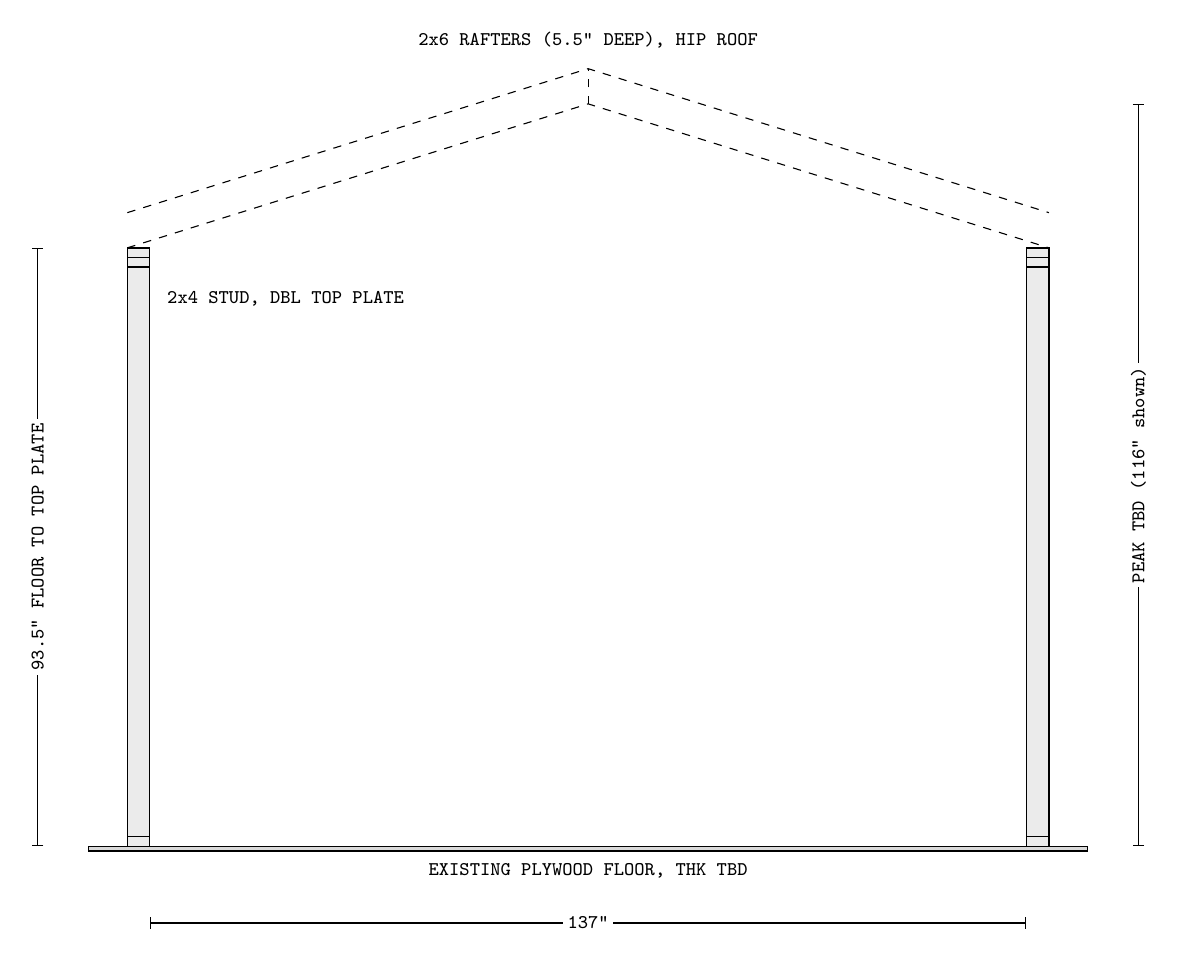
\begin{tikzpicture}[x=0.032in,y=0.032in]
\def\L{137}
\def\D{3.5}
\def\H{93.5}
\def\PK{116}
% floor
\fill[black!15] (-\D-6,-0.75) rectangle (\L+\D+6,0);
\draw[thin] (-\D-6,-0.75) rectangle (\L+\D+6,0);
% walls: plates + stud
\draw[wood] (-\D,0) rectangle (0,\H);
\draw[wood] (\L,0) rectangle (\L+\D,\H);
\draw[thin] (-\D,1.5) -- (0,1.5);   \draw[thin] (\L,1.5) -- (\L+\D,1.5);
\draw[thin] (-\D,\H-3) -- (0,\H-3); \draw[thin] (\L,\H-3) -- (\L+\D,\H-3);
\draw[thin] (-\D,\H-1.5) -- (0,\H-1.5); \draw[thin] (\L,\H-1.5) -- (\L+\D,\H-1.5);
% rafters 2x6 to assumed peak (dashed = assumed)
\draw[tbd] (-\D,\H) -- (\L/2,\PK) -- (\L+\D,\H);
\draw[tbd] (-\D,\H+5.5) -- (\L/2,\PK+5.5) -- (\L+\D,\H+5.5);
\draw[tbd] (\L/2,\PK) -- (\L/2,\PK+5.5);
% dims
\draw[dim] (-\D-14,0) -- (-\D-14,\H); \node[lab, rotate=90] at (-\D-14,\H/2) {93.5" FLOOR TO TOP PLATE};
\draw[dim] (\L+\D+14,0) -- (\L+\D+14,\PK); \node[lab, rotate=90] at (\L+\D+14,\PK/2) {PEAK TBD (116" shown)};
\draw[dim] (0,-12) -- (\L,-12); \node[lab] at (\L/2,-12) {137"};
\node[lab, anchor=west] at (2,\H-8) {2x4 STUD, DBL TOP PLATE};
\node[lab, anchor=south] at (\L/2,\PK+8) {2x6 RAFTERS (5.5" DEEP), HIP ROOF};
\node[lab, anchor=north] at (\L/2,-2) {EXISTING PLYWOOD FLOOR, THK TBD};
\end{tikzpicture}
\end{center}

\section{Door / Floor Raise}

\begin{center}
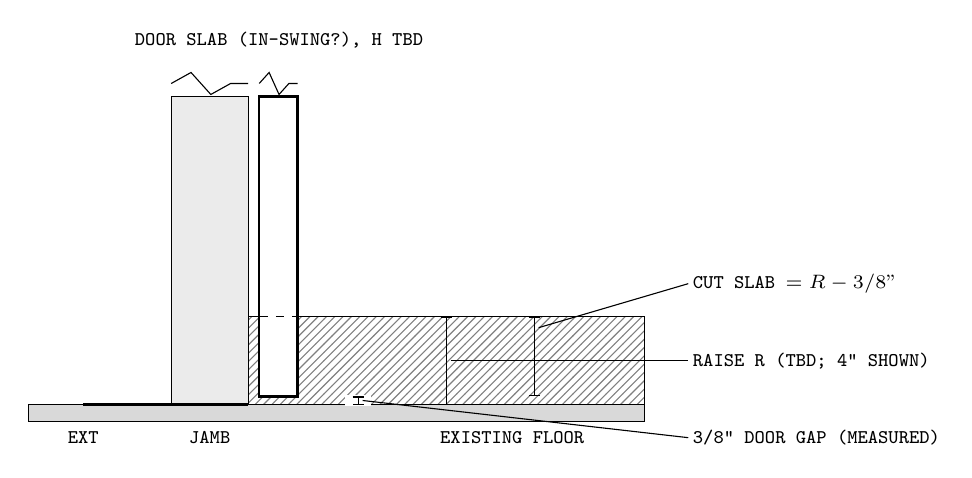
\begin{tikzpicture}[x=0.11in,y=0.11in]
\def\W{3.5}
\def\R{4}
% existing floor
\fill[black!15] (-10,-0.75) rectangle (18,0); \draw[thin] (-10,-0.75) rectangle (18,0);
% raised floor (hatched), R = 4 shown
\fill[pattern=north east lines, pattern color=black!50] (0,0) rectangle (18,\R);
\draw[thin] (0,0) rectangle (18,\R);
% jamb / wall, broken at top
\draw[wood] (-\W,0) rectangle (0,14);
\draw[thin] (-\W,14.6) -- ++(0.9,0.5) -- ++(0.9,-1) -- ++(0.9,0.5) -- ++(0.8,0);
% door slab, hangs 3/8 above existing floor
\draw[thick, fill=white] (0.5,0.375) rectangle (2.25,14);
\draw[tbd] (0.5,\R) -- (2.25,\R);
\draw[thin] (0.5,14.6) -- ++(0.45,0.5) -- ++(0.45,-1) -- ++(0.45,0.5) -- ++(0.4,0);
% threshold / exterior
\draw[thick] (-\W-4,0) -- (0,0);
% dims + leaders
\fill[white] (4.4,-0.05) rectangle (5.6,0.45); \draw[dim] (5,0) -- (5,0.375);   \draw[thin] (5.2,0.19) -- (20,-1.5); \node[lab, anchor=west] at (20,-1.5) {3/8" DOOR GAP (MEASURED)};
\draw[dim] (9,0) -- (9,\R);      \draw[thin] (9.2,\R/2) -- (20,2);    \node[lab, anchor=west] at (20,2) {RAISE R (TBD; 4" SHOWN)};
\draw[dim] (13,0.375) -- (13,\R);\draw[thin] (13.2,\R-0.5) -- (20,5.5);\node[lab, anchor=west] at (20,5.5) {CUT SLAB $= R - 3/8"$};
\node[lab, anchor=south] at (1.4,16) {DOOR SLAB (IN-SWING?), H TBD};
\node[lab, anchor=north] at (-\W/2,-1) {JAMB};
\node[lab, anchor=north] at (-\W-4,-1) {EXT};
\node[lab, anchor=north] at (12,-1) {EXISTING FLOOR};
\end{tikzpicture}
\end{center}

{\ttfamily\footnotesize
\begin{tabular}{@{}ll@{}}
Gap now & 3/8" \\
Any raise $R > 3/8"$ & in-swing door hits new floor; cut slab $R-3/8"$ or re-hang \\
Ceiling after raise & $93.5 - R$ \\
Door clear height after raise & slab H $- R + 3/8$ (slab H TBD) \\
\end{tabular}
}

\end{document}
